\documentclass{standalone}
\usepackage{tikz}
\usetikzlibrary{positioning}
\usepackage{graphicx}

\begin{document}
\begin{tikzpicture}[node distance=1.8cm, >=stealth, every node/.style={inner sep=0}]

% Define nodes with images
\node (A) {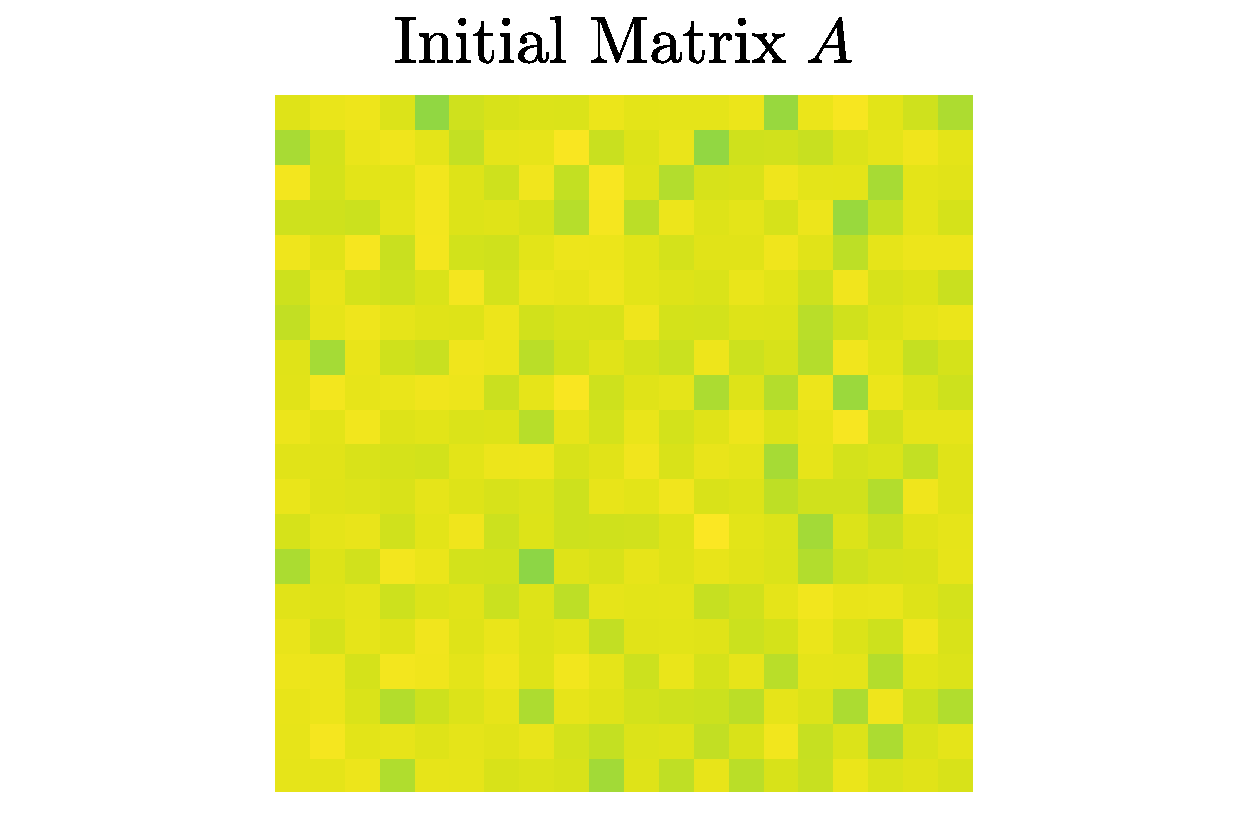
\includegraphics[width=10cm]{NormalJacobi_phase0.pdf}};
\node[right=of A, xshift = - 3cm] (B) {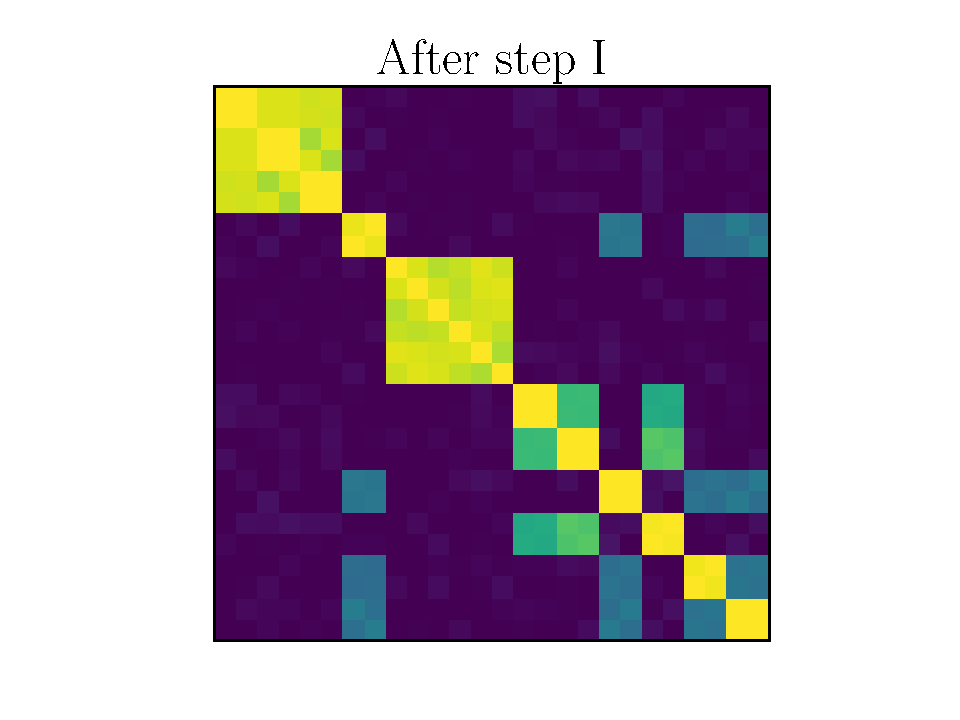
\includegraphics[width=10cm]{NormalJacobi_phase1.pdf}};
\node[right=of B, xshift=-3cm] (C) {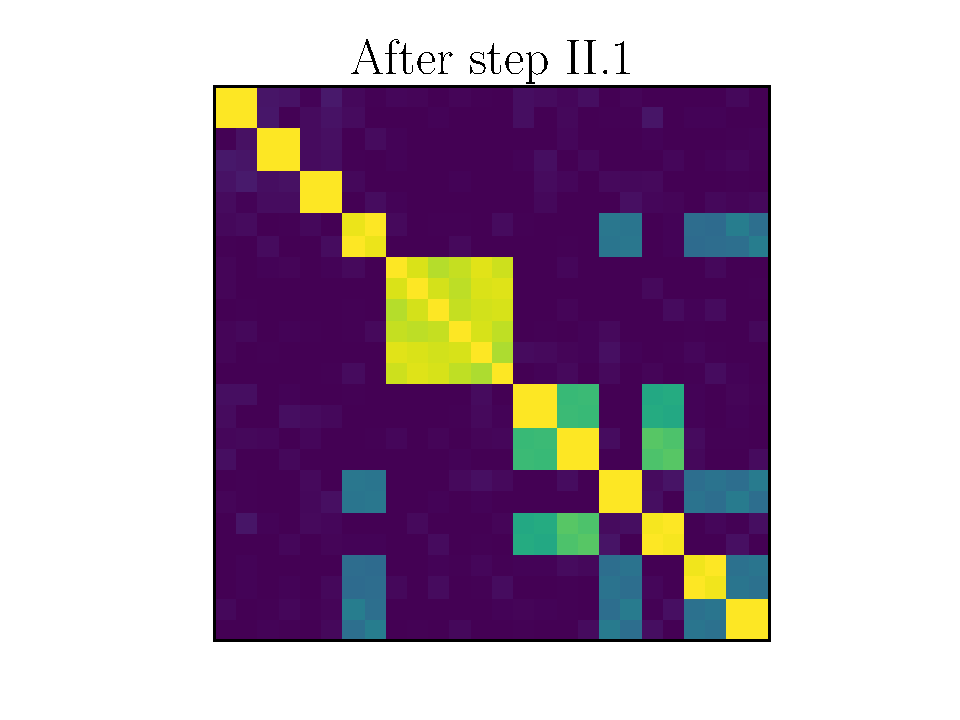
\includegraphics[width=10cm]{NormalJacobi_phase2.pdf}};

\node[below=of A, xshift=0cm] (D) {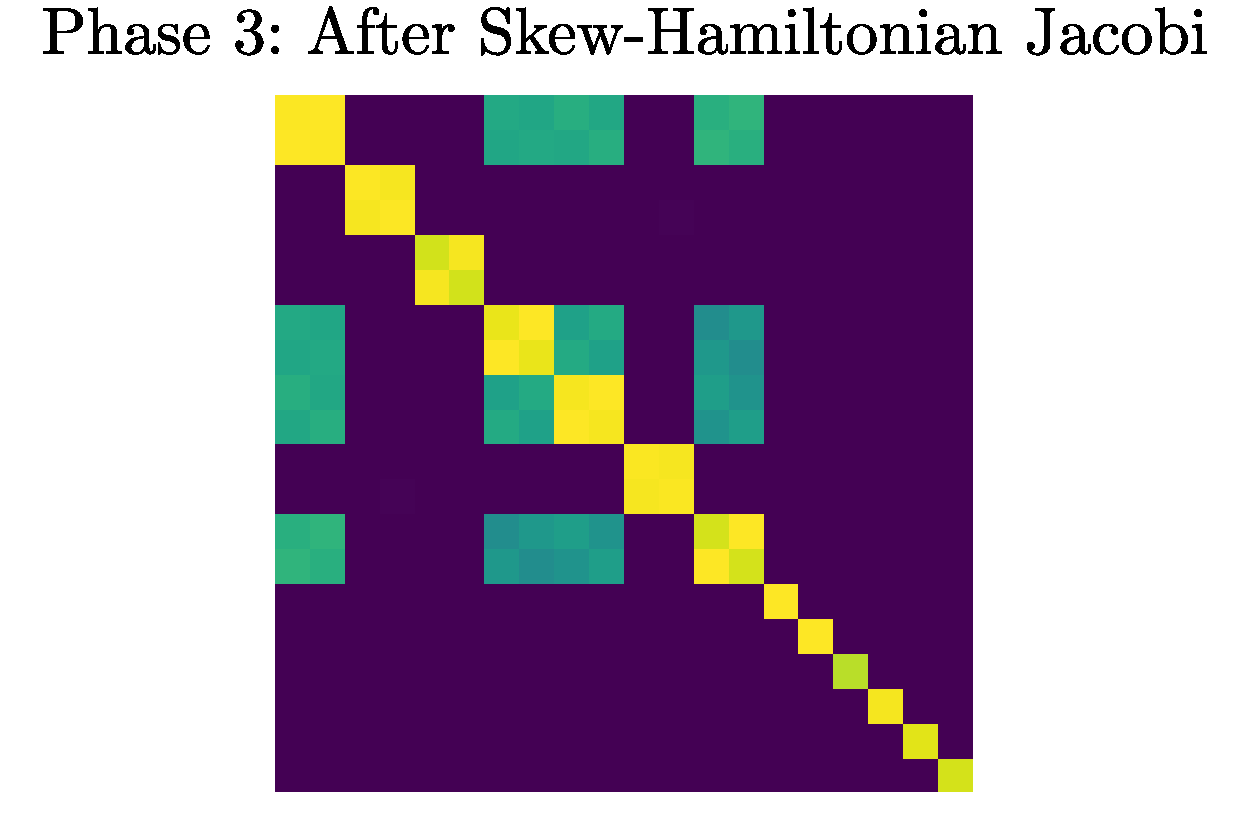
\includegraphics[width=10cm]{NormalJacobi_phase3.pdf}};
\node[below=of B, xshift=0cm] (E) {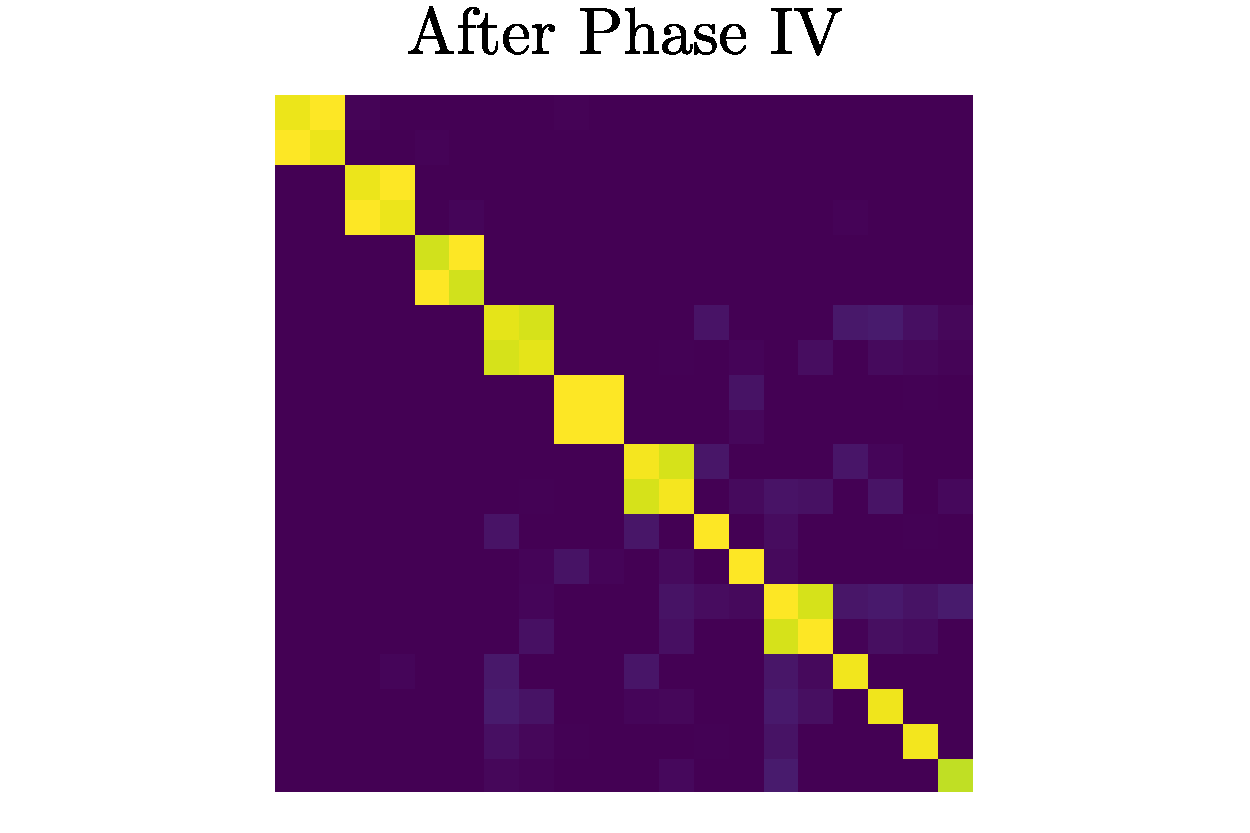
\includegraphics[width=10cm]{NormalJacobi_phase4.pdf}};
\node[below=of C, xshift=0.6cm] (F) {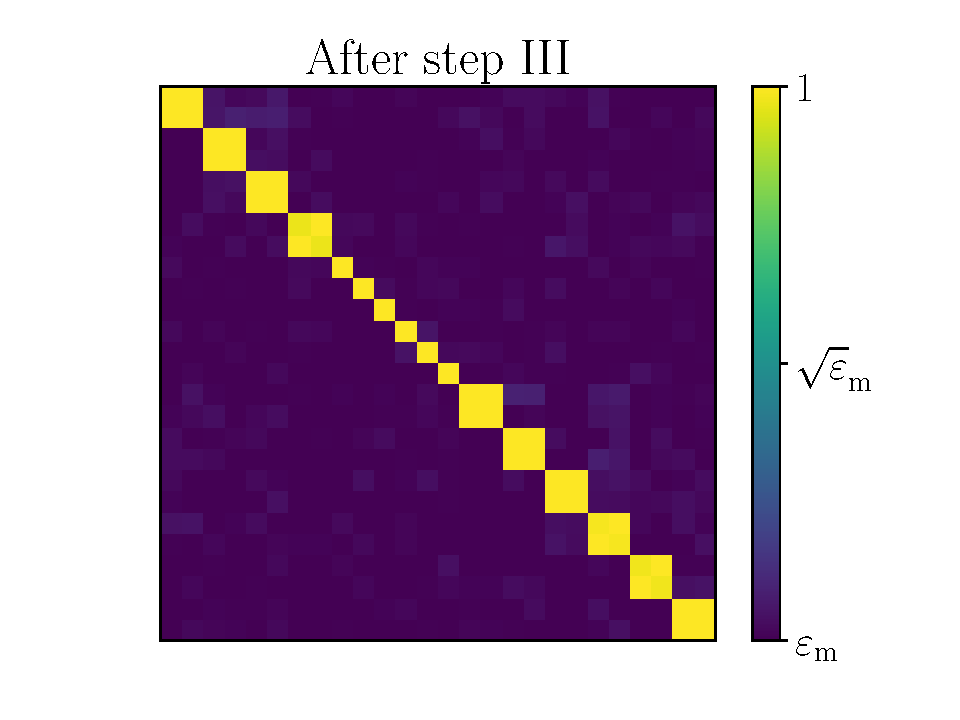
\includegraphics[width=10cm]{NormalJacobi_phase5.pdf}};

% Draw arrows to represent phases
\draw[->,thick] (B) -- (A);
\draw[->,thick] (C) -- (B);
%\draw[->,thick] (C) -- (D);
\draw[->,thick] (E) -- (D);
\draw[->,thick] (17.8,-3.6) --++ (0,-1) --++ (-17.8, 0) --++ (0,-1);
%\draw[->,thick] (E) --++ (0.1, 0);
\draw[->,thick] (12.7,-9.25) --++ (1.3, 0);

\end{tikzpicture}
\end{document}